\documentclass[oneside]{article}
 \headheight = 25pt
\footskip = 20pt
\usepackage{graphicx}

\usepackage{mdwlist}
\usepackage[T1]{fontenc}
\renewcommand{\rmdefault}{ppl}
\usepackage{fancyhdr}
 \pagestyle{fancy}
 \lhead{\textbf{\textsc{\small Scott O'Connor\\Metaphysics}}}
 \chead{}
 \rhead{\large\textbf{\textsc{Space}}}
 \lfoot{\footnotesize{\thepage}}
 \cfoot{}
 \rfoot{\footnotesize{\today}}
 \usepackage{longtable,booktabs}
\tolerance=700


\begin{document}
\thispagestyle{fancy}

\subsection*{Introduction}

This is a very introductory look at debates about the nature of space.
Our goals in this module:

\begin{enumerate}

\item
  Introduce and clarify the distinction between two theories of space,
  Absolutism and Relationalism, as well as briefly discuss how this
  debate is important for settling questions about the existence of
  vacua and absolute motion.
\item
  Introduce Kant's argument for Absolutism.
\item
  Consider how the existence of higher spatial dimensions affects Kant's
  argument (next week).
\end{enumerate}

We don't see space. We see objects that stand in spatial relations to
one another. One object is 10 feet from me. Another is 20 feet from me.
Being inaccessible to direct observation is unimportant. Neutrinos are
not directly observable either, but they still exist. Our question is
whether space has an independent existence from the objects that exist
in space and the relations they stand in to one another.

\begin{description}
\item[\textbf{Absolutism} (also called substantivalism):]
Space exists as an independent object in its own right over and above
the material content of the universe. Space is a continuous and
pervasive media that extends everywhere.
\item[\textbf{Relationalism:}]
Space does not exist as an independent object. There is only the
material content of the universe and the relations objects stand in to
one another. Space is merely defined through spatial relations among the
material objects in the universe.
\end{description}

\subsection*{Some Terminology}
\begin{description}
\item[\textbf{Properties}] are what objects exemplify (or instantiate)
individually or one by one, e.g., blue, red, angular, alive, etc.
\item[\textbf{Object:}] o is an object just if (i) there is some property P such that Po and
(ii) there is no x such that o is a property of x.\footnote{Some
  metaphysicians will prefer to use the word `particular' or
  `individual' in place of `object'. The terminological differences mask
  an important similarity; they all agree that there are beings which
  possess properties but are not themselves properties of anything else.} We can subsequently define different types of objects.
\begin{description}
\item[\textbf{Physical Object:}]
x is a physical object if (i) x is an object and (ii) x occupies some
region of space.
\item[\textbf{Abstract Object:}]
x is an abstract object if (i) x is an object and (ii) x does not occupy
a region of space.
\end{description}

\item[\textbf{Relations}] are exemplified by several individuals in relation to
each other, e.g., \emph{being a mile apart} is something that is
exemplified by a pair of objects---one thing is a mile away from
another. Similarly, \emph{being next to} is a spatial relation between
objects: one object is next to another. Relations have different features:

\begin{enumerate}
\item
  A relation R is \textbf{symmetrical} if, given any pair of objects a
  and b, \[ aRb \leftrightarrow bRa \]
\item
  A relation R is \textbf{asymmetrical} if, given any pair of objects a
  and b, \[ aRb\ \&\  \neg bRa\]
\item
  A relation R is \textbf{transitive} if, given some objects a, b, and
  c, \[ (aRb\ \&\ bRc) \rightarrow aRc \]
\item
  A relation R is \textbf{non-transitive} if, give some objects a, b,
  and c, \[ (aRb\  \&\  bRc)\ \& \neg aRc \]
\item
  A relation R is \textbf{reflexive} if for some object a, \[ aRa \]
\item
  A relation R is \textbf{non-reflexive} if some some object a,
  \[ \neg aRa \]
\end{enumerate}
\end{description}

\subsection*{Absolutism}
Absolutism is the view that space exists and is an abstract object.
\begin{quote}
Space is eternal in duration and immutable in nature\ldots{} Although
space may be empty of body, nevertheless it is itself not a void: and
something is there, because spaces are there, although nothing more than
that (\emph{De Gravitatione}, as quoted by Dainton, 133).
\end{quote}

\begin{quote}
Absolute space, in its own nature, without relation to anything
external, remains always similar and immovable (\emph{Principia}, as quoted
by Huggett, 118).
\end{quote}
Here are the most important claims the Absolutist makes:
\begin{enumerate}
\item Space exists as an abstract object.
\item There are absolute spatial relations like \emph{located at} between objects and places in space, e.g., Socrates can have an absolute location by standing in the relation of being located at to some region of space. 
\item Physical objects stands in absolute spatial relation, e.g., Suppose that X and Y are 10 feet apart. X is located in the region R1 of space that contains it. Y is located in the region R2 of space that contains it. Absolutism says that between R1 and R2 there exists another thing, a 10
foot region of space that separates X and Y.
\end{enumerate}

\section*{Relationalism}
Relationalism is the view that spatial relations exist but space itself
does not:

\begin{quote}
{[}T{]}he Mind can fancy to itself an Order made up of Genealogical
Lines, whose Bigness would consist only in the Number of Generations,
wherein every Person would have his Place. (The Leibniz-Clarke
Correspondence, (ed.) Alexander 1956, 70)
\end{quote}

\begin{quote}
and if to this one should add the Fiction of a Metempsychosis, and bring
in the same Human Souls again; the Persons in those Lines might change
place; he who was a Father, or a Grandfather, might become a Son, or a
Grand-son etc. (Ibid. 70-1)
\end{quote}

\begin{quote}
And yet those Genealogical Places, Lines, and Spaces, though they should
express real Truths, would only be Ideal Things. (Ibid. 71)
\end{quote}
Some of the most important claims of Relationalism:
\begin{enumerate}
\item Space does not exist as either an abstract of physical object, e.g., if X and Y are 10 feet apart and there is nothing in between
them, then there does not also exist the regions of
space that X and Y occupy as well as the region of space separating X and Y.
\item Spatial relations do exist, e.g., X and Y stand in the relation of being 10 feet apart.
\end{enumerate}
How might physical objects stand in spatial relations if space itself does not exist? Leibniz uses families as an example. A family is simply a group of people standing in certain relations to
each other: daughter, uncle, cousin, etc. The relations do exist. They are something
additional to the collection of individual people in the family. How about the family? Is the family
something in addition to these individuals and the relations they stand in to one another? Is it an
object in its own right that contains people, grows over time, etc? Leibniz says no.

Consider the sentence `my family has lived in Wexford for two
centuries'. The expression `the family' does not pick out some person
who has been alive for 200 years. We use the phrase to refer to a group
of people who stand in familial relations. Similarly, Leibniz thinks
that space is not a real object above and beyond the objects that it
supposedly contains. There are just the various spatial relations that
objects stand in to one another.



\subsection*{What is at stake?}\label{what-is-at-stake}

The debate between the Relationalist and Absolutist has been taken as
important for settling two issues:

\begin{enumerate}
\item
  Do vacua, empty spaces, exist?
\item
  Does absolute motion exist? 
\end{enumerate}
The Absolutist can answer `yes' to both questions. They can define a
vacua as an empty region of space (recall that they believe that space
really exists.) They can define Absolute Motion in terms of occupying
different regions of space at different times. The Relationalist is more
likely to answer `no' to both questions. They deny that there are empty spaces between two objects. They also are likely to claim that only relative motion exists, i.e., an object counts as moving only in relation to objects that are at rest.

\subsection*{Historical Precursors}\label{historical-precursors}

\begin{itemize}
\item
  Democritus (460--370 BC) vs.~Aristotle (384--322 BC) \emph{Physics, De
  Caelo}
\item
  Sir. Isaac Newton (1643--1727), \emph{Philosophia Naturalis Principia
  Mathematica} (1687) vs.~Gottfried Wilhelm Leibniz (1646--1716),
  \emph{The Leibniz-Clarke Correspondence} (1715--1716)
\end{itemize}

\subsection*{Incongruent Counterparts}\label{incongruent-counterparts}




Immanuel Kant (1724--1804) argued for Absolutism in \emph{Concerning the
Ultimate Foundation of the Differentiation of Regions of Space} (1768).
His main claims is that absolute space is necessary to explain the existence of
incongruent counterparts.

\begin{figure}[h]
  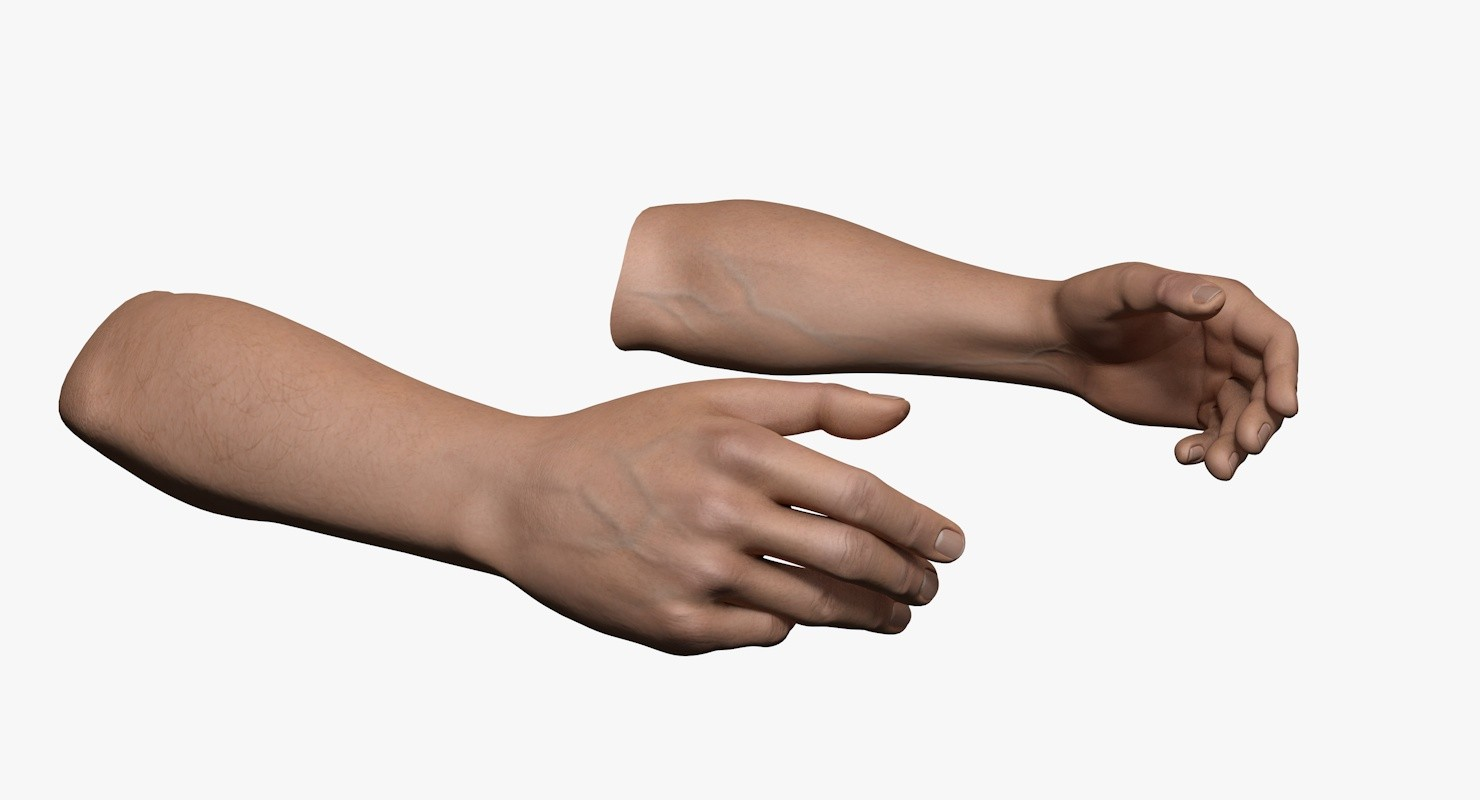
\includegraphics[width=\linewidth]{hands.jpg}
  \caption{Incongruent Counterpart}
\end{figure}

\begin{quote}
{[}An incongruent counterpart is{]}\ldots{}an object which is completely
like and similar to another, although it cannot be included exactly
within the same limits.
\end{quote}
There are two types of mirror objects. Let X be an object and let Y be
its mirror image.

\begin{enumerate}

\item
  X is a \textbf{congruent counterpart} of Y if X can be made to
  coincide with Y by rigid motions (without changing its shape or
  size).\footnote{If you know what a Mobius strip is, ignore the
    complication.}
\end{enumerate}

\begin{enumerate}

\item
  X is an \textbf{incongruent counterpart} of Y if X cannot be made to
  coincide with Y by rigid motions.
\end{enumerate}
An object is said to possess handedness just when it and its mirror
image are incongruent counterparts. An object is said to lack handedness just when it and its mirror image are congruent counterparts. Kant argues that the existence of handedness requires the existence of absolute space.

\subsection*{Master Argument}\label{master-argument}

The argument strategy: There are spatial differences between right and
left hands. We want to know what gives a hand one of these spatial
features as opposed to another. The reason why a giraffe is taller than
a mouse is that the height of the former is greater than the height of
the latter. Similarly, what is it about my left hand that makes it a
left hand as opposed to a right hand? We'll identify the only viable
options for explaining handedness and exclude all but one, Absolutism.

\begin{enumerate}

\item
  A hand is left or right either (a) solely in virtue of the
  \emph{internal} relations among the parts of the hand, or (b) at least
  partly in virtue of the \emph{external} relations of the hand to other
  material objects, or (c) in virtue of the \emph{external} relations of
  the hand to space itself.
\item
  Since the internal relations are the same for right and left, a hand
  is not left or right solely in virtue of its internal relations,
\item
  A hand is neither right nor left even partly in virtue of its
  relations to other material objects.
\item
  Therefore, a hand is left or right at least party in virtue of its
  relation to absolute space.\footnote{`Incongruent Counterparts and
    Higher Dimensions', by James Van Cleve}
\end{enumerate}

1--3 state the premises of the argument. 4 states the conclusion. The
argument is valid. If it is sound, then 4 must be true. Here are the
arguments for the premises.

\subsection*{P2. Internalism}\label{p2.-internalism}

Internalists accept 1 and 3, but they rejects 2. They accept that a hand
that was all alone in the Universe would still be a right or left hand,
but they think that it's being left or right can be explained without
looking outside the hand itself. The features of the hand alone, they
claim, will make it a right or left one. Hence, one needs no other
material objects or space itself to explain these features.

Objection:

\begin{enumerate}

\item
  The internal relations of both the left and right hand are distances
  between points and angles between lines, e.g., the length of the index
  finger.
\item
  The internal relations of both the left and right hand are identical.
\item
  If the internal relations of a right hand make it a right hand, then
  they cannot be identical to the internal relations of a left hand.\\
\item
  The internal relations of a right hand do not make it a right hand
  (similarly for the left hand)\ldots{}(from a--c)
\end{enumerate}

Our conclusion says that internal relations cannot distinguish right
from left handedness.

\subsection*{P3. Externalism}\label{p3.-externalism}

Externalists accept 1 and 2, but reject 3. They claim that being a left
or right hand depends on a relationship to other material objects. Kant
raises the following objection:

\begin{enumerate}

\item
  Suppose that there is a world in which only a hand, H, exists.
\item
  Suppose that a body possessing no hands pops into existence.
\item
  H can fit only the left or the right wrist.
\item
  If H fits the right wrist, H was a right hand before the body popped
  into existence.
\item
  If H fits the left wrist, H was a left hand before the body popped
  into existence.
\item
  H was a right or left hand before the body popped into
  existence\ldots{}(from c--e)
\item
  H was a right or left hand when no other material object
  exists\ldots{}(from f)
\item
  H's being a right or left hand is not explained by its relationship to
  any other material object\ldots{}(from g)
\end{enumerate}

\subsection*{Absolutism}\label{absolutism}

There were three candidates for explaining handedness. Internalism and
Externalism is false. The remaining candidate, Kant claims, Absolutism
must be true.

\end{document}
